% !TEX TS-program = XeLaTeX
% use the following command:
% all document files must be coded in UTF-8
\documentclass[spanish]{textolivre}
% build HTML with: make4ht -e build.lua -c textolivre.cfg -x -u article "fn-in,svg,pic-align"

\journalname{Texto Livre}
\thevolume{17}
%\thenumber{1} % old template
\theyear{2024}
\receiveddate{\DTMdisplaydate{2023}{7}{6}{-1}} % YYYY MM DD
\accepteddate{\DTMdisplaydate{2023}{8}{2}{-1}}
\publisheddate{\DTMdisplaydate{2023}{10}{31}{-1}}
\corrauthor{Ernesto Colomo}
\articledoi{10.1590/1983-3652.2024.46791}
%\articleid{NNNN} % if the article ID is not the last 5 numbers of its DOI, provide it using \articleid{} commmand 
% list of available sesscions in the journal: articles, dossier, reports, essays, reviews, interviews, editorial
\articlesessionname{articles}
\runningauthor{Aguilar-Cuesta et al.} 
%\editorname{Leonardo Araújo} % old template
\sectioneditorname{Hugo Heredia Ponce}
\layouteditorname{Thaís Coutinho}

\title{El papel de la tecnología educativa en las ciencias sociales: análisis bibliométrico}
\othertitle{O papel da tecnologia educacional nas ciências sociais: análise bibliométrica}
\othertitle{The role of educational technology in social sciences: bibliometric analysis}
% if there is a third language title, add here:
%\othertitle{Artikelvorlage zur Einreichung beim Texto Livre Journal}

\author[1]{Ángel Ignacio Aguilar-Cuesta~\orcid{0000-0003-3240-0810-2177}\thanks{Email: \href{aguilarcuesta@uma.es}{aguilarcuesta@uma.es}}}
\author[1]{Ernesto Colomo-Magaña~\orcid{0000-0002-3527-7937}\thanks{Email: \href{ecolomo@uma.es}{ecolomo@uma.es}}}
\author[1]{Julio Ruiz-Palmero~\orcid{0000-0002-6958-0926}\thanks{Email: \href{julioruiz@uma.es}{julioruiz@uma.es}}}
\affil[1]{Universidad de Málaga, Facultad de Ciencias de la Educación, Departamento de Didáctica y Organización Escolar, Málaga, España.}

\addbibresource{article.bib}
% use biber instead of bibtex
% $ biber article

% used to create dummy text for the template file
\definecolor{dark-gray}{gray}{0.35} % color used to display dummy texts
\usepackage{lipsum}
\SetLipsumParListSurrounders{\colorlet{oldcolor}{.}\color{dark-gray}}{\color{oldcolor}}

% used here only to provide the XeLaTeX and BibTeX logos
\usepackage{hologo}

% if you use multirows in a table, include the multirow package
\usepackage{multirow}

% provides sidewaysfigure environment
\usepackage{rotating}

% CUSTOM EPIGRAPH - BEGIN 
%%% https://tex.stackexchange.com/questions/193178/specific-epigraph-style
\usepackage{epigraph}
\renewcommand\textflush{flushright}
\makeatletter
\newlength\epitextskip
\pretocmd{\@epitext}{\em}{}{}
\apptocmd{\@epitext}{\em}{}{}
\patchcmd{\epigraph}{\@epitext{#1}\\}{\@epitext{#1}\\[\epitextskip]}{}{}
\makeatother
\setlength\epigraphrule{0pt}
\setlength\epitextskip{0.5ex}
\setlength\epigraphwidth{.7\textwidth}
% CUSTOM EPIGRAPH - END

% LANGUAGE - BEGIN
% ARABIC
% for languages that use special fonts, you must provide the typeface that will be used
% \setotherlanguage{arabic}
% \newfontfamily\arabicfont[Script=Arabic]{Amiri}
% \newfontfamily\arabicfontsf[Script=Arabic]{Amiri}
% \newfontfamily\arabicfonttt[Script=Arabic]{Amiri}
%
% in the article, to add arabic text use: \textlang{arabic}{ ... }
%
% RUSSIAN
% for russian text we also need to define fonts with support for Cyrillic script
% \usepackage{fontspec}
% \setotherlanguage{russian}
% \newfontfamily\cyrillicfont{Times New Roman}
% \newfontfamily\cyrillicfontsf{Times New Roman}[Script=Cyrillic]
% \newfontfamily\cyrillicfonttt{Times New Roman}[Script=Cyrillic]
%
% in the text use \begin{russian} ... \end{russian}
% LANGUAGE - END

% EMOJIS - BEGIN
% to use emoticons in your manuscript
% https://stackoverflow.com/questions/190145/how-to-insert-emoticons-in-latex/57076064
% using font Symbola, which has full support
% the font may be downloaded at:
% https://dn-works.com/ufas/
% add to preamble:
% \newfontfamily\Symbola{Symbola}
% in the text use:
% {\Symbola }
% EMOJIS - END

% LABEL REFERENCE TO DESCRIPTIVE LIST - BEGIN
% reference itens in a descriptive list using their labels instead of numbers
% insert the code below in the preambule:
%\makeatletter
%\let\orgdescriptionlabel\descriptionlabel
%\renewcommand*{\descriptionlabel}[1]{%
%  \let\orglabel\label
%  \let\label\@gobble
%  \phantomsection
%  \edef\@currentlabel{#1\unskip}%
%  \let\label\orglabel
%  \orgdescriptionlabel{#1}%
%}
%\makeatother
%
% in your document, use as illustraded here:
%\begin{description}
%  \item[first\label{itm1}] this is only an example;
%  % ...  add more items
%\end{description}
% LABEL REFERENCE TO DESCRIPTIVE LIST - END


% add line numbers for submission
%\usepackage{lineno}
%\linenumbers

\begin{document}
\maketitle

\begin{polyabstract}
\begin{abstract}
El desarrollo educativo de las Ciencias Sociales, donde destacan la geografía y la historia, es un terreno propicio para incorporar los avances tecnológicos con aplicabilidad al enriquecimiento de los procesos formativos y la mejora del interés y rendimiento del alumnado. Partiendo del interés del uso de la tecnología educativa en las ciencias sociales, el objetivo de este estudio es analizar con técnicas bibliométricas la producción científica en Scopus sobre dicho tema. Fue aplicada la declaración PRISMA, la muestra final la conforman 126 artículos publicados en las dos primeras décadas del siglo XXI, utilizando análisis bibliométricos de acoplamiento bibliográfico, coautoría, cocitación y co-ocurrencia. Los resultados señalan una producción en crecimiento pero de forma moderada, principalmente en revistas tanto de las ciencias sociales como de la tecnología. Destacan las investigaciones europeas, con redes colaborativas entre Reino Unido, Canadá y Australia, aunque España fue el país más prolífico. Dentro de las Ciencias Sociales, predominan los trabajos en torno a la geografía, siendo la materia con mayor desarrollo en las distintas etapas formativas (primaria, secundaria o universitaria). Recursos como los videojuegos o la realidad virtual y aumentada adquieren cada vez más protagonismo en los procesos formativos. Como conclusión, cabe destacar el impacto positivo de las tecnologías en el desarrollo educativo de las ciencias sociales y las diferentes líneas de investigación que se abren para un área de conocimiento propicia para la innovación.

\keywords{Ciencias sociales \sep Tecnologías \sep Educación \sep Estudio bibliométrico}
\end{abstract}

\begin{portuguese}
\begin{abstract}
O desenvolvimento educativo das Ciências Sociais, em que se destacam a Geografia e a História, é um terreno favorável à incorporação de avanços tecnológicos com aplicabilidade ao enriquecimento dos processos de formação e à melhoria do interesse e desempenho dos alunos. Partindo do interesse pelo uso da tecnologia educacional nas ciências sociais, o objetivo deste estudo é analisar com técnicas bibliométricas a produção científica na Scopus sobre tal tópico. Foi aplicada a declaração PRISMA e a amostra final é composta por 126 artigos publicados nas duas primeiras décadas do século XXI, utilizando análises bibliométricas de acoplamento bibliográfico, coautoria, cocitação e coocorrência. Os resultados indicam uma produção crescente, mas de forma moderada, principalmente em revistas tanto das ciências sociais como da tecnologia. Destaca-se a investigação europeia, com redes colaborativas entre o Reino Unido, Canadá e Austrália, embora a Espanha tenha sido o país mais prolífico. Nas Ciências Sociais predominam os trabalhos sobre Geografia, sendo a matéria com maior desenvolvimento nas diferentes etapas formativas (primária, secundária ou universidade). Recursos como videogames ou realidade virtual e aumentada adquirem cada vez mais destaque nos processos formativos. Concluindo, vale destacar o impacto positivo das tecnologias no desenvolvimento educacional das ciências sociais e das diferentes linhas de pesquisa que abrem uma área de conhecimento propícia à inovação.

\keywords{Ciências Sociais \sep Tecnologias \sep Educação \sep Estudo bibliométrico}
\end{abstract}
\end{portuguese}

\begin{english}
\begin{abstract}
The educational development of the Social Sciences, with a particular focus on geography and history, provides fertile ground for incorporating technological advancements with practical applications to enhance educational processes and improve student interest and performance. With the interest in the use of educational technology in the social sciences, the
objective of this study is to analyze the scientific production on this topic in Scopus using bibliometric techniques. It was applied the PRISMA statement, the final sample consists of 126
articles published in the first two decades of the 21st century, utilizing bibliometric analyses such as bibliographic coupling, co-authorship, co-citation, and co-occurrence. The results indicate a growing production but moderately, mainly in journals focused on both the social sciences and technology. European research stands out, with collaborative networks between the United Kingdom, Canada, and Australia, although Spain was the most prolific country. Within the Social Sciences, there is a predominance of studies in the field of geography, which is the subject with the most development across different educational stages (primary, secondary, and university). Resources such as video games or virtual and augmented reality are gaining increasing prominence in educational processes. In conclusion, the positive impact of technology on the educational development of the social sciences and the various lines of research that emerge in this knowledge field, conducive to innovation, should be highlighted.

\keywords{Social Sciences \sep Technologies \sep Education \sep Bibliometric study}
\end{abstract}
\end{english}
% if there is another abstract, insert it here using the same scheme
\end{polyabstract}

\section{Introducción}

A lo largo de las últimas décadas, hemos visto cómo la entrada de la tecnología se iba
abriendo paso dentro la sociedad, afectando de lleno a la educación \cite{colomo2023acultural, guillen2023adigital}. El desarrollo de las Tecnologías de la Información y la
Comunicación (TIC en adelante) ha mejorado el proceso de enseñanza-aprendizaje \cite{moreno2022computer}, convirtiéndose en una herramienta cada vez más usada por docentes \cite{guillen2023bconstruccion, pintosantos2023formacion} y discentes \cite{rodriguez2022competencia} y dando lugar a nuevas metodologías que tuvieron un punto de inflexión durante la
pandemia de COVID-19, al tener que transformar la presencialidad por el aprendizaje virtual
\cite{aguilar, oguguo2023analysis}.

Estas estrategias, métodos o recursos digitales \cite{colomo2023binstantaneas, colomomagana2023cpercepcion, lopez2023aaugmented, lopez2023bmetaverse, marin2021steam}, se han integrado dentro de las
materias curriculares, aunque con distinto grado de desarrollo, tanto por las materias en sí mismas, como por los contenidos y diversidad de estas. Para el caso que nos ocupa, las
Ciencias Sociales, debemos advertir primeramente que engloba a varias disciplinas: Historia, Geografía, Historia del Arte, Filosofía en algunas etapas educativas, etc., con toda la diversidad y subdisciplinas en las que cada una se subdividen. Esto hace que la variedad de contenidos temáticos a tratar sea amplia, permitiendo a las TIC un mayor espacio para converger con ellas dentro del aula \cite{araya2022didactica}.

Sin embargo, se ha producido un desarrollo desigual en el uso de las TIC dentro de la materia de Ciencias Sociales, existiendo una escasa atención por parte de los investigadores a principios del s. XXI. Esta debilidad, según apunta \textcite{gomez2019investigacion}, se debe a la consideración de la didáctica de las Ciencias Sociales como un área sin consenso en el cuerpo teórico y unos métodos y técnicas que debían mejorarse, ya que a finales del s. XX se contaba con escasos análisis e investigaciones que permitieran un crecimiento sostenido de la investigación en didáctica de las Ciencias Sociales \cite{prats2002hacia}.


No obstante, debemos advertir que esas disciplinas no han tenido el mismo crecimiento respecto a la implementación de tecnologías. Según los análisis realizados hasta la fecha, las publicaciones se han centrado mucho más en investigación que en experiencias y propuestas didácticas o en reflexiones teóricas \cite{alonso22, mcdougall2006theory}. Además, las áreas y temáticas también muestran altas diferencias, ya que la educación histórica y patrimonial, supera ampliamente a la didáctica de la geografía, historia del arte o el resto de subdisciplinas que engloba el término ciencias sociales. En este sentido, las TIC juegan un papel minoritario, como también lo hace la evaluación \cite{martinez2021} y la formación del profesorado, encontrando estudios centrados en el uso de aplicaciones concretas para la realización de tareas \cite{aguilar2022covid}. Aquí cabe prestar atención a la formación inicial de los docentes, contexto donde debería germinarse la unión entre tecnología educativa y su aplicación en el área curricular de ciencias sociales. En España, esta demanda se materializa en un trabajo de la Universidad de Navarra \cite{ciriza2022technological}, cuyo propósito fue que los futuros docentes desarrollaran la competencia digital en la enseñanza de las ciencias sociales mediante la integración de los tipos de conocimiento tecnológico, pedagógico y de contenido utilizando el modelo TPACK. Con 235 estudiantes del Grado en Educación Primaria, trabajando en una asignatura de Historia, los hallazgos señalan que poseen una autopercepción positiva sobre su competencia digital y que desarrollar propuestas formativas sobre Historia con TIC tiene efectos positivos. Con 646 docentes de Historia en formación para la etapa de Educación Secundaria en España, la investigación de \cite{gomez2022recursos}, se centró en analizar el estilo de enseñanza y el uso de recursos digitales en un aula. Los resultados reflejaron que, en líneas generales, hay un vínculo débil entre los recursos digitales y los procesos educativos desarrollados. En Turquía, encontramos que la concienciación medioambiental se beneficia del uso de medios TIC. Así ocurre con 323 futuros maestros de ciencias sociales \cite{sadik2014study}, valorando el 43\% positivamente el uso de la televisión e internet como recurso en el proceso educativo por su influencia beneficiosa en la conciencia ambiental. 

Esto pone de manifiesto el tipo de Ciencias Sociales que se enseña, mucho más teórica que digital, a pesar de que los avances tecnológicos permiten utilizar medios que mejoran el proceso formativo \cite{jdaitawi2022factors, olivas2022strategic}, permitiendo conocer, por ejemplo, el estado del tiempo, el precio de alquileres o ventas de viviendas, o calcular rutas y destinos a los que ir.

Se hace preciso, por tanto, conocer con mayor nivel de profundidad las distintas experiencias, intervenciones y trabajos que han implementado las tecnologías, desde una perspectiva educativa, para el desarrollo de los procesos de enseñanza-aprendizaje en el área de ciencias sociales en las dos primeras décadas del siglo XXI. Vinculado a ello, el objetivo de esta investigación es analizar bibliométricamente la producción científica sobre el uso educativo de las TIC en ciencias sociales en la base de datos internacional Scopus.

Partiendo de dicho propósito, se especifican varias preguntas de investigación:

\begin{itemize}
    \item ¿Cuál ha sido el desarrollo de la producción científica sobre el uso educativo de las TIC en ciencias sociales atendiendo a las variables año, áreas de conocimiento, revistas, país, afiliación y publicaciones más relevantes? 
    \item ¿Qué autores son los responsables de los artículos más influyentes en el ámbito académico? 
    \item ¿En torno a qué países se establecen las principales redes de colaboración más prolíficas sobre la temática contemplada? 
    \item ¿Cuáles son las principales líneas de investigación dentro del ámbito de estudio?

\end{itemize}


\section{Metodología}

Para abordar el propósito y las preguntas antes expuestas, se realizó un estudio bibliométrico. Se trata de implementar técnicas de metaanálisis respecto a la producción científica objeto de estudio \cite{gonzalez2020quality}, considerando un conjunto de directrices y criterios para realizar los análisis precisos a tenor de las variables establecidas, con un enfoque cuantitativo e interpretativo \cite{civico2022twitter}. Su validez queda sustentada por los múltiples estudios que realizaron siguiendo este método \cite{boulahrouz2018digital, colomo2020spoc, colomo2022mooc, lopez2021co, mielgo2022revision, moreno2019estudio, ruiz2021revision}.

Los documentos fueron seleccionados tomando como referencia la base de datos Scopus. El motivo de su elección radicó en que posee una producción científica suficientemente amplia y sometida a rigurosos criterios de calidad \cite{khanra2020big}. Las palabras claves y boleanos que se introdujeron en el comando de búsqueda fueron "Information technology and communication" OR "Educative technology" OR "ICT" AND "social sciences" OR "geography" OR "history" AND “Education” OR “teaching” OR “learning” OR “pedagogy”. La búsqueda contempló título, palabras claves y resúmenes, reportando un total de 739 documentos, encontrándose entre ellos artículos, libros, capítulos, ponencias o editoriales.

A partir de los 739 documentos resultantes, se emplearon diversos criterios de cribado (\Cref{fig1}) a tenor del fenómeno de estudio, cumpliendo para ello con la declaración “Preferred Reporting Items for Systematic Reviews and Meta-Analyses”, conocido a nivel científico más por el acrónimo (PRISMA). El marco PRISMA favorece una estructura y organización que ayuda a los autores a dar a conocer mejor su proceso de revisión implementado \cite{garcia2022developing}.

\begin{figure}[h!]
\centering
\begin{minipage}{.8\textwidth}
 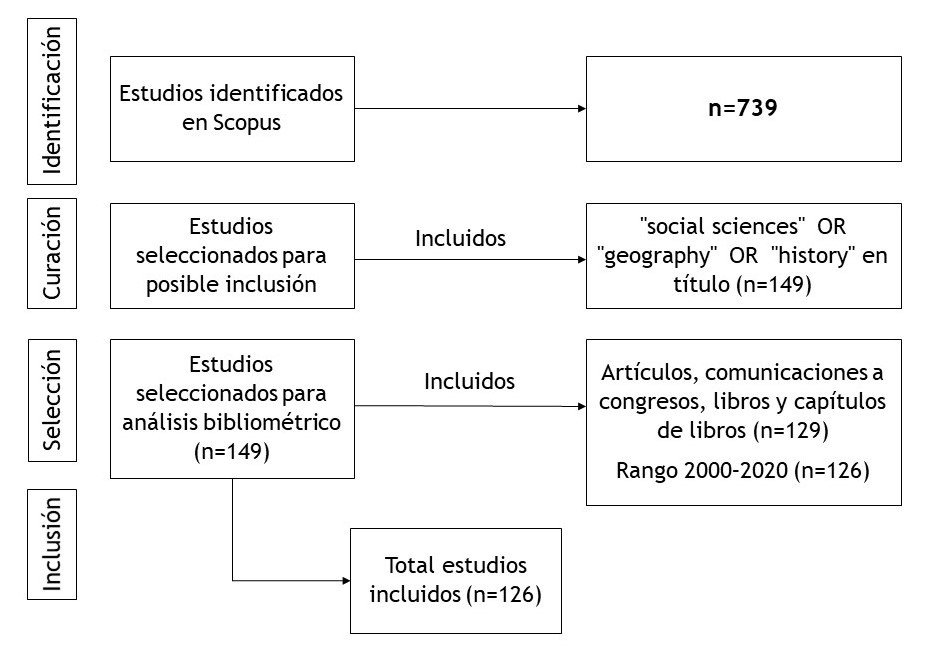
\includegraphics[width=\textwidth]{fig1.jpg}
 \caption{ Diagrama de flujo del proceso de selección de estudios basado en la declaración \emph{PRISMA}}
 \label{fig1}
 \source{Elaboración propia}
\end{minipage}
\end{figure}

En primer lugar, tras revisar los resúmenes de los documentos resultantes, se percibió que la inclusión de los comandos en los campos contemplados (título, resumen y palabras claves) incluían publicaciones no acordes con el objeto de estudio en el que se había situado el foco. Esto llevó a una modificación parcial en el motor de búsqueda, de forma que el comando de descriptores relacionados con las ciencias sociales ("social sciences" OR "geography" OR "history") cumpliera con la condición de aparecer en el título de la publicación. Esta restricción redujo la muestra a 145 documentos.  

Tras ello, se excluyeron de los resultados de la búsqueda los documentos que no eran artículos, comunicaciones a congresos, libros o capítulos de libro, con la consiguiente reducción de la muestra a 129 documentos. Por otra parte, se incluyeron todos los documentos que, cumpliendo el filtro anterior, han sido publicados en el rango 2000-2020, obviando los que se publicaron antes del inicio del milenio y los publicados con posterioridad, para cumplir el objetivo de estudio. De este modo, tras aplicar los diferentes filtros, la muestra final la conforman 126 documentos (76 artículos, 29 comunicaciones a congresos, 14 capítulos de libros y 7 libros), donde predominan las publicaciones en inglés (109), español (9) y esloveno (6). Los resultados fueron exportados en valores separados por comas (.csv) para el posterior análisis de la muestra con técnicas bibliométricas.

Para el análisis se utilizaron diversas técnicas de análisis bibliométrico: 

\begin{enumerate}
[label=\alph*)]
    \item producción científica, para explorar la evolución de dicha producción a tenor de se las variables determinadas;
    \item acoplamiento bibliográfico, para saber qué nivel de influencia tiene un artículo en el ámbito científico en base a su semejanza (referencias compartidas) con otras publicaciones afines;
    \item coautoría, para examinar las colaboraciones existentes respecto al tema de estudio, teniendo a los países como unidad de análisis en este estudio;
    \item  co-citación, para conocer la frecuencia con la que diferentes artículos se citan conjuntamente;
    \item co-ocurrencia, para identificar las palabras claves que más se utilizan en los artículos objeto de estudio. 
    
\end{enumerate}

El estudio de los nodos relacionales que se conformaron entre los artículos de la muestra, se desarrolló con el programa VOSviewer, un software de libre uso aunque no de código abierto, que permite construir y visualizar redes bibliométricas, representando los mapas de relaciones que se originan a nivel de acoplamiento bibliográfico, coautoría, co-citación y co-ocurrencia.

Atendiendo al análisis de la producción científica, se estipularon las variables siguientes: año, para explorar la evolución de los artículos en el tiempo; área de conocimiento, para saber en qué ámbitos temáticos se indexan los artículos; revistas, para identificar las publicaciones más prolíficas respecto al objeto de interés de este trabajo; país, para saber en qué países se investiga más sobre el fenómeno de estudio; afiliación, para examinar las instituciones que tienen una mayor producción; publicaciones con más impacto, para conocer cuáles eran los artículos más relevantes en el ámbito de estudio en el momento de realizar la investigación. No todos los resultados han sido considerados, sino que se establecieron criterios de exclusión en función de las variables consideradas, los cuales se especifican a continuación (\Cref{tab1}).

\begin{table}[h!]
\centering
\begin{threeparttable}
\caption{Variables de estudio y criterios de exclusión}
\label{tab1}
\begin{tabular}{ll}
\toprule
Variables                     & Criterios de exclusión                               \\
\midrule
Año                           & Todas las publicaciones fuera del rango 2000-2020    \\
Área de conocimiento          & Todas las áreas con menos de 10 publicaciones        \\
Revistas                      & Todas las revistas con menos de 3 artículos          \\
País                          & Todos los países con menos de 4 publicaciones        \\
Afiliación                    & Todas las instituciones con menos de 4 publicaciones \\
Publicaciones con más impacto & Todas las publicaciones con menos de 20 citas    \\
\bottomrule
\end{tabular}
\source{Elaboración propia}
\end{threeparttable}
\end{table}

\section{Análisis y resultados}

Con el propósito de acometer el análisis sobre la temática de estudio, se han organizado los resultados en función de las diferentes técnicas bibliométricas aplicadas, dando así respuesta a las preguntas de investigación. Se comienza por el análisis de la producción científica, para continuar con el acoplamiento bibliográfico, la coautoría, la co-citación y la co-ocurrencia.

\subsection{Análisis de la producción científica}

Partiendo de las 126 publicaciones que conformaron la muestra, se examinaron las diversas variables que fueron seleccionadas para el estudio.

\subsubsection{Año}

Considerando que se incluyeron las publicaciones dentro del rango 2000-2020 (\Cref{fig2}), ambos incluidos, se observa una evolución discontinua, con continuos crecimientos y descensos, generándose un rango de 16 publicaciones entre el año más productivo (17 en 2019) y que menos documentos registró (2001 con 1). De todos modos, si se aprecia un aumento de la producción en el periodo más reciente (2010-2020), respecto al periodo inicial estudiado (2000-2010).

\begin{figure}[h!]
\centering
\begin{minipage}{.8\textwidth}
 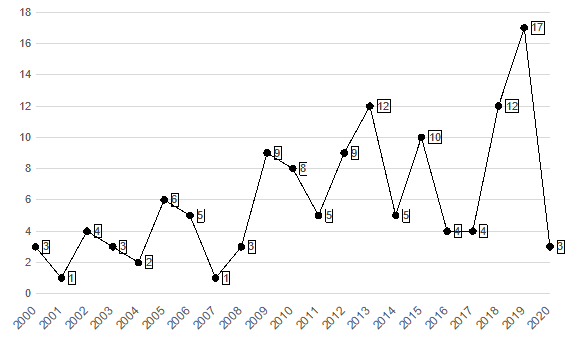
\includegraphics[width=\textwidth]{fig2.png}
 \caption{Artículos publicados por años}
 \label{fig2}
 \source{Elaboración propia}
\end{minipage}
\end{figure}

\subsubsection{Área de conocimiento}

En esta variable, el criterio de exclusión establecido fue no alcanzar las 10 publicaciones. Además, es preciso matizar que las publicaciones, respecto a su inclusión en las áreas de conocimiento, están supeditadas a un criterio de multiclasificación, dando lugar a que una misma publicación, dependiendo del tema abordado, pueda registrarse en una o varias áreas temáticas. Este hecho conlleva que la suma de todas las áreas en las que se registran publicaciones (\Cref{tab2}) sea superior a los 126 documentos que forman la muestra final.

\begin{table}[h!]
\centering
\begin{threeparttable}
\caption{Área de conocimiento}
\label{tab2}
\begin{tabular}{ll}
\toprule
Área                        & Número de publicaciones \\
\midrule
Social Sciences             & 100                     \\
Computer Science            & 44                      \\
Earth and Planetary Science & 17                      \\
Engineering                 & 12                      \\
Arts and Humanities         & 11                     \\
\bottomrule
\end{tabular}
\source{Elaboración propia}
\end{threeparttable}
\end{table}

El área de ciencias sociales registró la mayor producción (100), siendo más del doble que la de ciencias de la computación que, con 44 publicaciones, ocupa el segundo lugar. Llamó la atención la pluralidad en las áreas, diferenciándose dos ámbitos: los campos de conocimiento más arraigados a los contenidos de sociales (ciencias sociales, ciencias de la tierra y el planeta, artes y humanidades); y el ámbito tecnológico, al tener la variable TIC y tecnología educativa como herramienta/instrumento vehiculado al proceso educativo sobre las materias de sociales.


\subsubsection{Revista}

Partiendo del criterio de exclusión estipulado de menos de 3 publicaciones sobre la temática de análisis (\Cref{tab3}), el primer lugar lo ocupa la revista Geografía V Soli, del ámbito de las ciencias sociales. Vinculado a este terreno, también encontramos otras publicaciones como Journal Of Geography In Higher Education o Library Philosophy and Practice. El resto están vinculadas al campo de la tecnología, como ya ocurriera en las áreas de indexación. Cabe destacar que, pese a que España es el país más prolífico en cuanto a producción sobre el tema, ninguna de las revistas es española, debido en gran parte al menor número de estas indexadas en Scopus y en posiciones relevantes respecto a métricas de impacto.

\begin{table}[h!]
\centering
\begin{threeparttable}
\caption{Revistas indexadas en Scopus con mayor número de publicaciones}
\label{tab3}
\begin{tabular}{ll}
\toprule
Nombre revista                                     & Número de publicaciones \\
\midrule
Geografija V Soli                                  & 5                       \\
Journal Of Geography In Higher Education           & 4                       \\
Communications In Computer And Information Science & 3                       \\
Computers And Education                            & 3                       \\
Library Philosophy And Practice                    & 3                       \\
\bottomrule
\end{tabular}
\source{Elaboración propia}
\end{threeparttable}
\end{table}

\subsubsection{País}

Tener menos de 4 publicaciones sobre la temática objeto de estudio (\Cref{tab4}) fue el criterio de exclusión para la variable país.

\begin{table}[h!]
\centering
\begin{threeparttable}
\caption{Países con más publicaciones en Scopus}
\label{tab4}
\begin{tabular}{ll}
\toprule
País           & Número de publicaciones \\
\midrule
España         & 24                      \\
Reino Unido    & 22                      \\
Grecia         & 10                      \\
Eslovenia      & 7                       \\
Australia      & 6                       \\
Estados Unidos & 5                       \\
Finlandia      & 4                       \\
Suráfrica      & 4                       \\
\bottomrule
\end{tabular}
\source{Elaboración propia}
\end{threeparttable}
\end{table}

España lideró la producción científica, atendiendo a los comandos de búsqueda establecidos, seguida de cerca por Reino Unido (24 y 22, respectivamente). Existe un predominio mayoritario de países europeos entre los más prolíficos, no encontrado hasta la 5º posición a Australia con 6 publicaciones. También aparecen del continente americano (Estados Unidos, con 5 publicaciones) y el africano (Suráfrica, con 4), aunque con pocas publicaciones si consideramos todos los años que fueron considerados para el estudio.


\subsubsection{Afiliación}

Al igual que en la variable país, para considerar las instituciones de afiliación se establecieron registrar un mínimo de 4 publicaciones (\Cref{tab5}), encontrando solo 4 universidades que cumplen dicho criterio.

\begin{table}[h!]
\centering
\begin{threeparttable}
\caption{Instituciones con más publicaciones en Scopus}
\label{tab5}
\begin{tabular}{ll}
\toprule
Institución      & Número de publicaciones \\
\midrule
University of East Anglia & 4                                \\
Universidad de Murcia     & 4                                \\
University of Strathclyde & 4                                \\
Universidad de Salamanca  & 4                                \\
\bottomrule
\end{tabular}
\source{Elaboración propia}
\end{threeparttable}
\end{table}

Cabe señalar que dichas instituciones son universidades de los dos países más prolíficos (España y Reino Unido), algo lógico si consideramos los resultados de la variable anterior. Entre dichas instituciones, la universidad de Salamanca y Murcia comparten primera posición con 4 publicaciones, al igual que las de East Anglia y Strathclyde.


\subsubsection{Publicaciones con más impacto}

En lo que respecta a las publicaciones más relevantes, en función del número de citas, se excluyeron los documentos publicados que tenían menos de 20 citas totales (\Cref{tab6}). 

%TABELA6 

\begin{table}[htbp]
\centering
\begin{threeparttable} 
    \small
    \caption{Publicaciones con más impacto en Scopus}
    \label{tab6}
    \begin{tabular}{p{3cm}lp{4cm}p{3cm}ll}
      \toprule
      Autores & Año & Título & Revista & Citas & \multicolumn{1}{p{1cm}}{Media de citas por año} \\
      \midrule
      Tüzün, H., Yilmaz-Soylu, M., Karakuş, T., Inal, Y., Kizilkaya, G. & 2009 & The effects of computer games on primary school students' achievement and motivation in geography learning & Computers and Education, 52(1), 68-77 & 331 & 27.6 \\[13ex]
      Maqsood, T., Finegan, A., Walker, D. & 2006 & Applying project histories and project learning through knowledge management in an Australian construction company & Learning Organization, 13(1), 80-95 & 41 & 2.7 \\[3ex]
      Lynch, K., Bednarz, B., Boxall, J., Chalmers, L., France, D., Kesby, J. & 2008 & E-learning for geography's teaching and learning spaces & Journal of Geography in Higher Education, 32(1), 135-149 & 30 & 2.3 \\[3ex]
      Favier, T.T., Van Der Schee, J.A. & 2014 & The effects of geography lessons with geospatial technologies on the development of high school students' relational thinking & Computers and Education, 76, 225-236 & 26 & 3.7 \\[3ex]
      McDougall, A., Jones, A. & 2006 & Theory and history, questions and methodology: Current and future issues in research into ICT in education? & Technology, Pedagogy and Education, 15(3), 353-360 & 25 & 1.7 \\[3ex]
      Mendler, J., Simon, D., Broome, P. & 2002 & Virtual development and virtual geographies: Using the Internet to teach interactive distance courses in the global South & Journal of Geography in Higher Education, 26(3), 313-325 & 20 & 1.1 \\
         \bottomrule
    \end{tabular}
    \source{Elaboración propia}
\end{threeparttable}
\end{table}

La publicación más relevante es la de \textcite{tuzun2009effects}, logrando las 331 citas y un promedio de 27.6 citas por año. Este estudio se centró en una experiencia con videojuegos en educación primaria para la enseñanza de geografía, demostrando que la utilización de dicho recurso TIC mejoró el rendimiento académico del alumnado y su motivación intrínseca. Vinculado a la temática específica de la geografía, encontramos otras 3 publicaciones. Por un lado, relacionadas con el contexto universitario, el trabajo de \textcite{favier2014effects} apuesta por técnicas geoespaciales para la mejora de dicho pensamiento en estudiantes de educación superior; mientras que el estudio de \textcite{mendler2002virtual}, analizó los pro y contras de un programa formativo de postgrado online en Geografía respecto a su diseño tecno-pedagógico, organizativo y de accesibilidad del alumnado. Por otra parte, \textcite{lynch2008learning} fundamentan la implementación de las TIC para la enseñanza de la geografía a todos los niveles. Subrayar que el segundo lugar, con 41 citas, lo ostentó la investigación de \textcite{maqsood2006applying}, donde las TIC favorecían el aprendizaje basado en proyectos para empresas mediante el trabajo sobre análisis históricos de los proyectos en desarrollo. De una forma más general, \textcite{mcdougall2006theory} defendían el papel de las TIC en el desarrollo de los procesos formativos, encontrándose las ciencias sociales entre sus contenidos. 


\subsection{Acoplamiento bibliográfico}

La aplicación de esta técnica permitió subrayar la relevancia de un artículo, dentro de la muestra de trabajos contemplados, a partir de su vínculo y semejanza con otras publicaciones. Concretamente, se atendió al número de referencias compartidas entre las publicaciones objeto de estudio, empleando un encadenamiento de citas, permitiendo identificar a los autores más significativos en relación con el uso educativo de las TIC para el ámbito de las ciencias sociales. Se aplicó como unidad de análisis los autores para el acoplamiento bibliográfico, estipulando como criterios un mínimo de 1 documento y de 25 citas por autor. 10 ítems cumplieron con el criterio, reflejándose en la \Cref{fig3} los nodos generados. 

 Se generaron 3 conjuntos de autorías en función del acoplamiento entre los mismos. El clúster rojo tiene la mayor intensidad de acoplamiento (total link strenght 157), generada en torno a la publicación de \textcite{tuzun2009effects}, al ser el documento con más citas compartidas. En el lado opuesto, los clústers azul y verde alcanzan ambos la menor intensidad (total link strenght 59), siendo la diferencia que la publicación enmarcada en el conjunto azul \cite{favier2014effects} tiene más citas (26) que la publicación del conjunto verde \cite{mendler2002virtual}, con 20 citas. De este modo, son 3 publicaciones las que sientan las bases de las referencias bibliográficas sobre las que se construyen el resto de las publicaciones.

\begin{figure}[h!]
\centering
\begin{minipage}{.9\textwidth}
 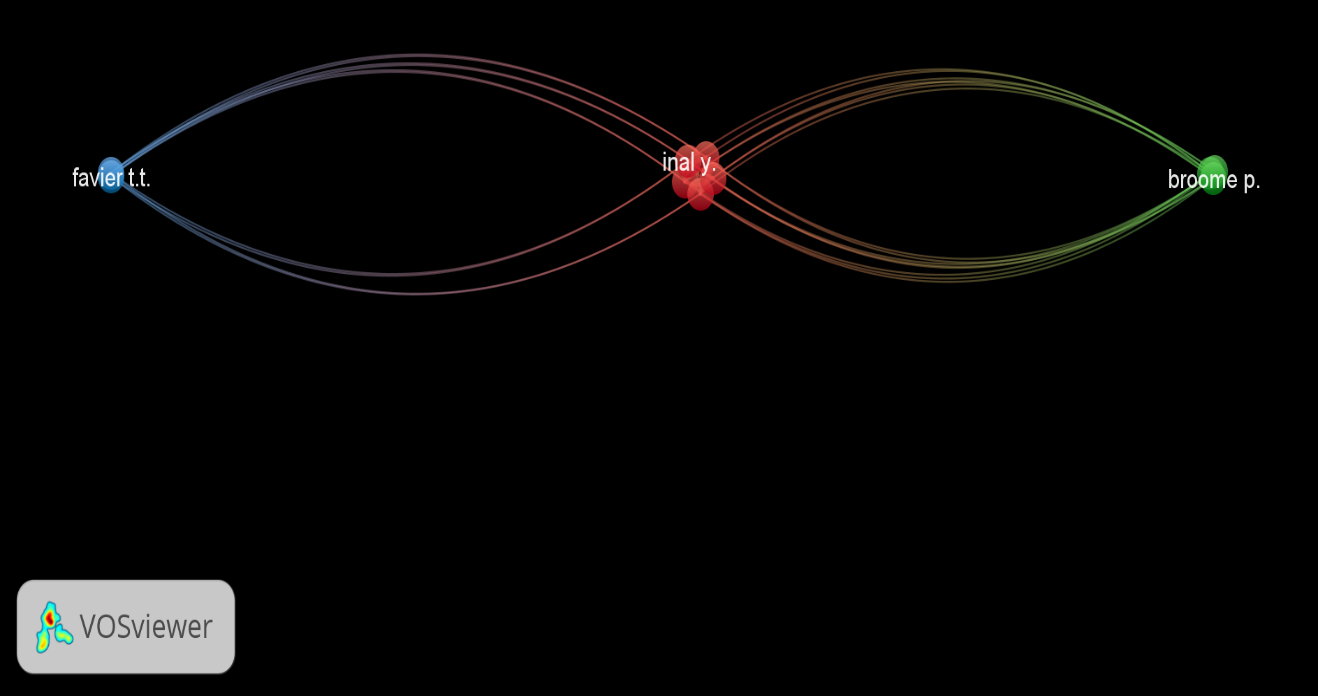
\includegraphics[width=\textwidth]{fig3.png}
 \caption{Acoplamiento bibliográfico con “autores” como unidad de análisis}
 \label{fig3}
 \source{Elaboración propia}
\end{minipage}
\end{figure}


\subsection{Análisis coautoría}

Para conocer las redes colaborativas existentes entre países sobre la producción científica objeto de estudio, se aplicó un análisis de coautoría. Se incluyeron aquellos países con al menos 2 publicaciones en coautoría que tuvieran un mínimo de 20 citas. Un total de 6 países cumplieron dicho criterio, tal y como se refleja en la \Cref{fig4}.

\begin{figure}[h!]
\centering
\begin{minipage}{.9\textwidth}
 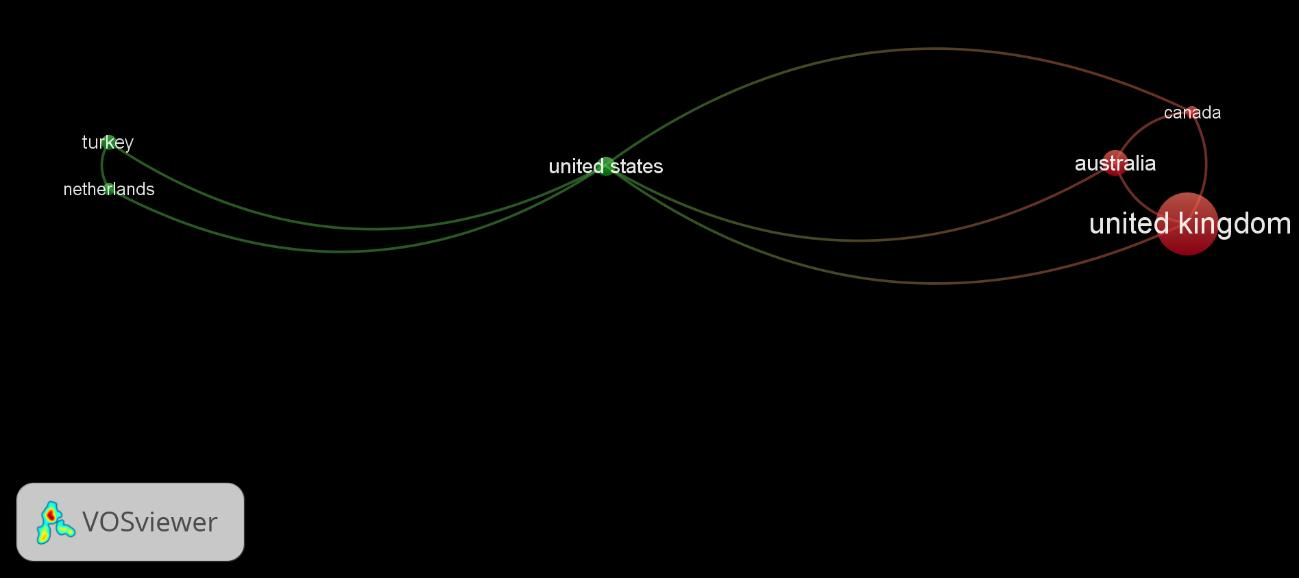
\includegraphics[width=\textwidth]{fig4.jpg}
 \caption{Coautoría con “países” como unidad de análisis}
 \label{fig4}
 \source{Elaboración propia}
\end{minipage}
\end{figure}

Se generaron 2 clústers en función de las coautorías, precisando aclarar que el tamaño de los nodos es consecuencia de su importancia, siendo mayor a medida que esta crece. Reino Unido, Australia y Canadá manifiestan una colaboración estrecha entre los mismos (clúster rojo), al igual que sucede en el conjunto verde (Turquía, Países Bajos y Estados Unidos). Señalar que Estados Unidos se convierte en el país con la mayor red de colaboración al vincularse con todos los que superan el filtro estipulado. También es relevante indicar que países con los registros de producción más altos, como España (24 publicaciones), Grecia (10) o Eslovenia (7), no establecen redes colaborativas relevantes (al menos 2 publicaciones con un mínimo de 20 citas como criterio para su inclusión) para la investigación en el objeto de estudio. De este modo, la colaboración entre países no queda sujeto a un mayor nivel de producción, sino a la generación de sinergias e intereses investigadores compartidos entre los autores. 



\subsection{Análisis de co-citación y co-ocurrencia}

Para abordar las principales líneas de investigación en torno a la aplicación educativa de las TIC en contenidos de ciencias sociales, se implementaron dos técnicas bibliométricas: análisis de co-citación, atendiendo a la frecuencia con la que publicaciones diferentes fueron citadas conjuntamente; análisis de co-ocurrencia de palabras claves, centrado en la frecuencia de aparición conjunta de los diferentes descriptores contemplados. 

Atendiendo a la co-citación, el criterio estipulado fue registrar un mínimo de 6 citas, cumpliéndolo 59 ítems (\Cref{fig5}). Se conformaron 4 conjuntos de co-citaciones, a tenor de las publicaciones que aparecen citadas a la vez. Cabe denotar la intensidad de co-citación de Lambert (total link strenght 2749), Piotrowska (total link strenght 1881) Cichon (total link strenght 1701) o Slater (total link strenght 1512). Esto nos permite comprobar como los trabajos de estos autores se han convertido en referencia en el campo de las ciencias sociales y las TIC para el resto de autores que han abordado dicha temática en sus trabajos, convirtiéndose así en lo que podría denominarse como publicaciones relevantes del área.

\begin{figure}[h!]
\centering
\begin{minipage}{.9\textwidth}
 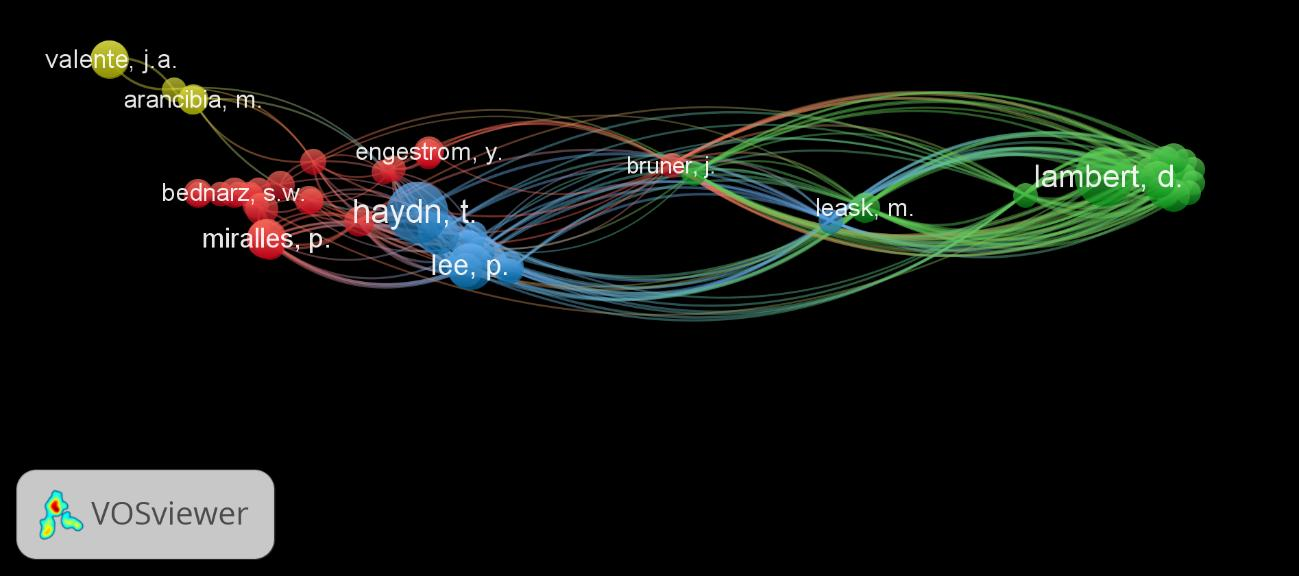
\includegraphics[width=\textwidth]{fig5.jpg}
 \caption{Co-citación con “autores” como unidad de análisis}
 \label{fig5}
 \source{Elaboración propia}
\end{minipage}
\end{figure}

En lo que respecta a la co-ocurrencia de los descriptores, de las 126 publicaciones que conformaron la muestra, los autores propusieron 350 palabras clave y los documentos se indexaron con 389 palabras clave, sumando un total de 628. De entre las mismas, 25 palabras claves concurrieron un mínimo de 5 veces (\Cref{fig6}). Se crearon 3 conjuntos, a partir de los descriptores que coexistieron como palabras clave.

\begin{figure}[h!]
\centering
\begin{minipage}{.9\textwidth}
 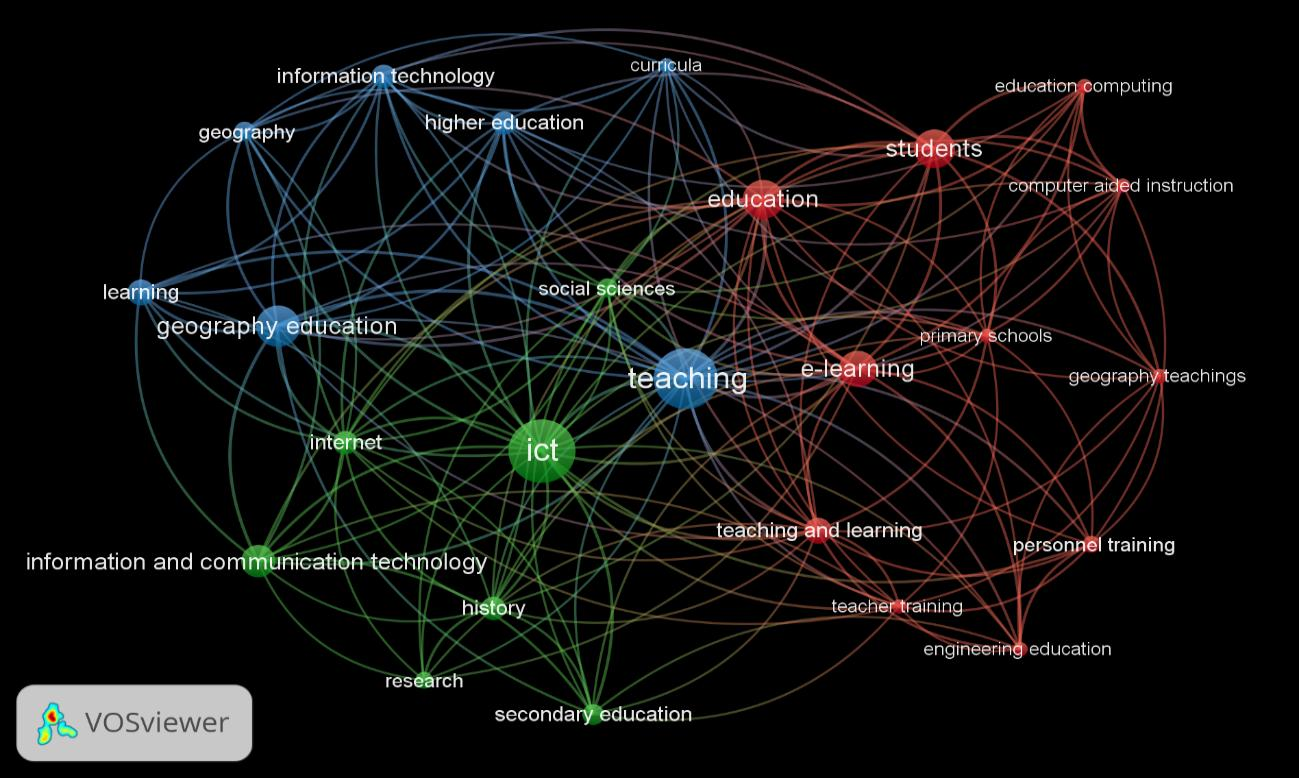
\includegraphics[width=\textwidth]{fig6.jpg}
 \caption{Concurrencia de palabras claves en la producción científica}
 \label{fig6}
 \source{Elaboración propia}
\end{minipage}
\end{figure}

Entre las palabras claves más frecuentes destacan descriptores introducidos en los comandos de búsqueda utilizados (ICT, 28; teaching, 27; geography education, 17). La presencia del término estudiante (16) evidencia el agente al que se dirigieron los esfuerzos en este ámbito temático. Cabe subrayar el papel del e-learning (15) para el desarrollo de los procesos formativos, las etapas educativas más habituales (educación superior, 9; educación secundaria, 8; educación primaria, 5) y otros ámbitos de aplicación como son la investigación (6), o la formación del profesorado (5). Estos hallazgos nos permiten, desde una doble perspectiva, conocer las principales líneas que se venían trabajando hasta la fecha analizada, y vislumbrar potenciales temáticas a desarrollar en futuros trabajos para reforzar los conocimientos sobre esta área de estudio.


\section{Discusión y conclusiones}
El trabajo bibliométrico ha subrayado una producción científica no excesivamente desarrollada sobre el uso educativo de las tecnologías en el ámbito de las ciencias sociales, con un margen amplio para el crecimiento, la difusión y la creación de redes colaborativas. 

Como se ha podido comprobar en los análisis, el objeto de estudio presenta una evolución discontinua respecto a la proliferación de publicaciones, primando las indexadas en ciencias sociales y ciencias de la computación. Las revistas referentes se dividen entre las propias del campo de las ciencias sociales y las relacionadas con las TIC, siendo esto debido al propio fin de analizar el impacto de las tecnologías en los procesos formativos del área objeto de estudio. Debemos reseñar también que predominaron las publicaciones de países europeos, generando entre España y Reino Unido el 36\% de estas, siendo sus universidades (Murcia, Salamanca, East Anglia y Strathclyde) las más prolíficas. Las publicaciones más relevantes (mayor número de citas) giran, principalmente, en torno a la geografía y cómo las tecnologías pueden mejorar los procesos de enseñanza-aprendizaje \cite{favier2014effects, lynch2008learning, mendler2002virtual, tuzun2009effects}. 

Si atendemos a los autores más influyentes, encontramos el trabajo de \textcite{tuzun2009effects}, enfocado en el papel de los videojuegos para la mejora del rendimiento y la motivación en el estudio de la geografía. También son relevantes los trabajos de \textcite{favier2014effects} y \textcite{mendler2002virtual}, ambos contextualizados en la etapa universitaria y el estudio de la geografía, dirigido, el primero, al desarrollo del pensamiento geoespacial, mientras que el segundo se centra en las posibilidades de un postgrado online sobre dicha materia.

Respecto a las redes colaborativas generadas entre países, en torno a investigadores cuya afiliación es una institución de Estados Unidos se produce el mayor número de colaboraciones, mientras que la más prolífica surge de la unión de investigadores de Reino Unido, Australia y Canadá. Significativo es que España, pese a ser el país con el mayor número de publicaciones, sus investigadores no han sido prolíficos en cuanto a colaboraciones con sus homónimos de otros países.

En cuanto a las principales líneas de investigación, los análisis de co-citación y co-ocurrencia refrendan la preferencia por la disciplina de la geografía, dentro de las ciencias sociales, como materia para el desarrollo de procesos educativos mediados por tecnologías, influyendo en estos resultados los boleanos seleccionados. Cabe reseñar los trabajos que reflejan el cambio en el paradigma del proceso formativo de la materia de geografía al incorporar las TIC \cite{hillis2005ict, piotrowska2019challenges, svobodova2016model}; las posibilidades que el e-learning han brindado para desarrollar los programas educativos sobre ciencias sociales \cite{bosco2011virtual, lynch2008learning, mendler2002virtual}; o su aplicación en diferentes etapas educativas, como primaria \cite{deaney2009case, grigoriou, villena2019strolling}, secundaria \cite{arancibia2013caracterizacion, arancibia2015concepciones, biddulph, garcia2015aproximacion} o universitaria \cite{miralles2019digital, ortega2019massive}.

Por todo ello, este trabajo supone subrayar el estado actual de la tecnología educativa y su impacto en el área curricular de las ciencias sociales desde comienzos del siglo XXI. Si bien hay publicaciones que respaldan este campo, los hallazgos reflejan falta de concreción respecto a línea de trabajo, enfoque de las investigaciones, potenciales colaboraciones e interés explícito y fehaciente por mejorar con las TIC las disciplinas que integran las ciencias sociales. Los principales trabajos son acercamientos de expertos en el área de ciencias sociales a las posibilidades que las tecnologías ofrecen para mejorar su praxis docente y factores claves del aprendizaje y formación de su alumnado como motivación o rendimiento. Sin embargo, falta crear sinergias que vinculen líneas de investigación más prolíficas con el uso de herramientas digitales que supongan una verdadera mejora para la formación en ciencias sociales, apostando por trabajos con amplias muestras sometidos a pre-test y post-test, o con grupos control y experimental. Solo de este modo podremos comprobar la validez y fiabilidad de las acciones didácticas con TIC en este terreno curricular.

Como implicaciones teóricas, este trabajo permite un análisis bibliométrico de la producción científica sobre las ciencias sociales y las TIC, pudiendo ser referente para posteriores trabajos que quieran seguir desarrollando el impacto que la tecnología educativa tiene en el desarrollo de una de las áreas curriculares más relevantes a nivel académico por la cantidad de disciplinas que la conforman. A nivel práctico, supone visibilizar quiénes son los autores, países e instituciones que más están investigando sobre esta área y en qué temas están centrando sus trabajos. De este modo, potenciales investigadores interesados en centrar sus labores investigadoras en este campo de conocimiento, puedan generar sinergias o dirigirse a equipos de trabajo con experiencia contrastada.

Para terminar, es preciso considerar las limitaciones de este trabajo, como es el hecho de la no inclusión de publicaciones de la base de datos Web of Science. En este sentido, los criterios de calidad que establece Scopus aseguran una muestra representativa, junto a evitar duplicidades y los consiguientes procesos de depuración a los que habría que someter a la muestra. En lo que concierne a posibles líneas de investigación futura, sería interesante complementar este estudio bibliométrico con una revisión bibliográfica, realizando un análisis documental que permita un mayor nivel de profundidad sobre este ámbito de conocimiento. Por igual, también podríamos conocer el impacto de las tecnologías en los procesos formativos en otras áreas y disciplinas, como las ciencias naturales, la literatura o las matemáticas.



\printbibliography\label{sec-bib}
% if the text is not in Portuguese, it might be necessary to use the code below instead to print the correct ABNT abbreviations [s.n.], [s.l.]
%\begin{portuguese}
%\printbibliography[title={Bibliography}]
%\end{portuguese}


%full list: conceptualization,datacuration,formalanalysis,funding,investigation,methodology,projadm,resources,software,supervision,validation,visualization,writing,review
\begin{contributors}[sec-contributors]
\authorcontribution{Ángel Ignacio Aguilar-Cuesta}[conceptualization,resources,methodology,writing,review]
\authorcontribution{Ernesto Colomo-Magaña}[conceptualization,datacuration, investigation,validation]
\authorcontribution{Julio Ruiz-Palmero}[formalanalysis,supervision,review]
\end{contributors}




\end{document}

